%!TEX root = ../../common/main.tex

\section{Backgrounds}
\label{sec:measurement_of_sin2beta:physic_backgrounds}

This section describes the evaluation of background contributions in the data.
Besides combinatorial background from particles combined by chance with
properties that allow to pass all selection steps two other sources are
investigated: physics backgrounds from decays with mis-identified final state
particles are studied in
\cref{sec:measurement_of_sin2beta:physic_backgrounds:physic_backgrounds} and the
influence of non-uniform tagging responses for the background candidates is
examined in
\cref{sec:measurement_of_sin2beta:physic_backgrounds:tagging_asymmetries}.

% ------------------------------------------------------------------------------
\subsection{Physics backgrounds}
\label{sec:measurement_of_sin2beta:physic_backgrounds:physic_backgrounds}

To ensure that the background consists only of combinatorial backgrounds, and
that exclusive backgrounds are negligible, possible physics backgrounds are
studied with simulated data (see
\cref{sec:measurement_of_sin2beta:data_preparation:datasamples:mc}).

Using the true particle identities from \MC reveals the existence of remnants
from physics backgrounds in the $\inclJPsi$ and the $\BdToJpsiX$ \MC samples.

Compared to the number of all reconstructed events, around $\SI{0.04}{\percent}$
$\BdToJpsiKstar$ candidates survive the applied selection criteria compared to
$\SI{0.5}{\percent}$ signal events in the sample of $\BdToJpsiX$ decays. In the
$\inclJPsi$ sample $\SI{0.0005}{\percent}$ $\BdToJpsiKstar$,
$\SI{0.0002}{\percent}$ $\BsToJpsiKS$, and $\SI{0.0002}{\percent}$
$\LbToJpsiLambda$ background events contribute, compared to
$\SI{0.01}{\percent}$ $\BdToJpsiKS$ candidates.

Since the production of $\Bs$ mesons is a factor $\num{100}$ less frequent than
that of the lighter $\Bd$ mesons and reconstructed $\BsToJpsiKS$ candidates lie
outside the nominal mass range, no contributions are expected. While
$\BdToJpsiKstar$ background results from kaon-pion mis-identification,
$\LbToJpsiLambda$ candidates are found in the sample due to a proton-pion
mis-identification. Their expected contribution in the data sample is further
studied by using signal \MC samples of $\BdToJpsiKstar$ and $\LbToJpsiLambda$.

\subsubsection{Physics backgrounds from $\mathbfsfit{\kaon}$-$\mathbfsfit{\pion}$ mis-ID}
\label{sec:measurement_of_sin2beta:physic_backgrounds:physic_backgrounds:kstar}

In the $\BdToJpsiKstar$ signal \MC $\SI{0.3}{\percent}$ of $\num{4e6}$ generated
background candidates get reconstructed and survive the applied stripping cuts.
This number already reduces to $\SI{0.004}{\percent}$ after applying cuts on the
nominal mass and time ranges. After full offline selection, considering a
tagging efficiency of $\SI{38}{\percent}$, and scaling the numbers to match a
data sample corresponding to
$\SI[separate-uncertainty=true]{3}{\per\femto\barn}$ integrated luminosity,
$\num{20}$ $\BdToJpsiKstar$ candidates remain. This corresponds to a fraction of
roughly $\SI{0.04}{\percent}$ of the background in the nominal data sample. The
source of the remaining contributions are \eg decays like
$\decay{\Bdstar}{\Bd(\to\jpsi\Kstarz)\,\Xparticle}$.

\subsubsection{Physics backgrounds from $\mathbfsfit{\proton}$-$\mathbfsfit{\pion}$ mis-ID}
\label{sec:measurement_of_sin2beta:physic_backgrounds:physic_backgrounds:lambda}

Out of $\num{3e6}$ generated $\LbToJpsiLambda$ signal candidates only
$\SI{2}{\percent}$ get reconstructed and pass the stripping. The cuts on the
nominal mass and time ranges reduce this number down to $\SI{0.32}{\percent}$.
The veto cut applied in the offline selection (see
\cref{sec:measurement_of_sin2beta:data_preparation:offline_selection:daughters})
decreases the number of candidates inside this mass and decay time window by
more than $\SI{50}{\percent}$ to $\SI{0.15}{\percent}$. After applying the full
offline selection, including the tagging efficiency, and scaling the sample to
correspond to the collected integrated luminosity in data, $\num{120}$
$\LbToJpsiLambda$ candidates remain. Therefore, we expect a $\SI{0.2}{\percent}$
contribution of $\LbToJpsiLambda$ background candidates in the nominal data
sample.

% ------------------------------------------------------------------------------
\subsection{Background tagging asymmetries}
\label{sec:measurement_of_sin2beta:physic_backgrounds:tagging_asymmetries}

As shown in the previous section any physics induced background in the data
sample can be neglected and the remaining background candidates are assumed to
be purely of combinatorial origin. Following this, all flavour tagging decisions
provided for background candidates should be randomly distributed. This
assumption can be tested in two ways: counting the time-integrated numbers of
\Bd and \Bdbar tagged background candidates or checking for a non-vanishing
time-dependent tag asymmetry in the background.

The tests are performed independently for the \catDD and \catLL sub sample as
well as for both employed tagging algorithms (\OS and \SSpi). In order to study
the background sample an unbinned maximum likelihood fit is performed on the \Bd
mass distribution and background \sWeights \cite{Pivk:2004ty} are computed. The
signal component is modelled using an Ipatia \PDF while the background component
is described by an exponential \PDF (\cf
\cref{sec:measurement_of_sin2beta:likelihood_fit:model:mass}).

% ..............................................................................
\subsubsection{Time integrated background asymmetry}
\label{sec:measurement_of_sin2beta:physic_backgrounds:tagging_asymmetries:time_integrated}

The time-integrated asymmetry
%
\begin{equation}\label{eq:measurement_of_sin2beta:physic_backgrounds:tagging_asymmetries:time_integrated}
  \Asym{\Bkg}{\text{int}} = \frac{N_{\Bkg}^{\Bdbar} - N_{\Bkg}^{\Bd}}{N_{\Bkg}^{\Bdbar} + N_{\Bkg}^{\Bd}}
\end{equation}
%
is computed for all four sub samples using the \sweighted dataset and the
results are collected in
\cref{tab:measurement_of_sin2beta:physic_backgrounds:tagging_asymmetries:time_integrated}. 
Compared to the time-integrated \CP asymmetry (\cf 
\cref{eq:measurement_of_sin2beta:systematics:cross_checks:time_integrated:cp_asym}) 
in the signal component in the order of $\order{\num{0.1}}$ the time-integrated
background tagging asymmetry is small and except for the \catDD \OS subsample
the results are not significant. A vanishing time-integrated asymmetry does not
eliminate the possibility of a time-dependent asymmetry, thus further studies
are necessary.
%
\begin{table}[h]
  \centering
  \caption{Time-integrated asymmetry of \sweighted background distributions for
  \catDD and \catLL \OS and \SSpi tagged events.}
  \label{tab:measurement_of_sin2beta:physic_backgrounds:tagging_asymmetries:time_integrated}
  \sisetup{
    table-number-alignment    = center,
    table-figures-integer     = 1,
    table-figures-decimal     = 3,
    table-figures-uncertainty = 3,
    table-sign-mantissa,
  }
  \begin{tabular}{llS}
    \toprule
    \multicolumn{2}{c}{category}           & {$\Asym{\Bkg}{\text{int}}$}\\
    \midrule
    \multirow{2}{*}{\catDD} & \acs*{OS}    &  0.017 +- 0.005 \\
                            & \acs*{SSpi}  & -0.016 +- 0.011 \\
    \multirow{2}{*}{\catLL} & \acs*{OS}    & -0.005 +- 0.012 \\
                            & \acs*{SSpi}  &  0.044 +- 0.034 \\
    \bottomrule
  \end{tabular}
\end{table}

% ..............................................................................
\subsubsection{Decay time dependent background asymmetry}
\label{sec:measurement_of_sin2beta:physic_backgrounds:tagging_asymmetries:time_dependent}

The decay time dependent background tagging asymmetry is defined similar to 
\cref{eq:measurement_of_sin2beta:physic_backgrounds:tagging_asymmetries:time_integrated} as
%
\begin{equation}\label{eq:measurement_of_sin2beta:physic_backgrounds:tagging_asymmetries:time_dependent}
  \Asym{\Bkg}{}(\obsTime) = \frac{N_{\Bkg}^{\Bdbar}(\obsTime) - N_{\Bkg}^{\Bd}(\obsTime)}{N_{\Bkg}^{\Bdbar}(\obsTime) + N_{\Bkg}^{\Bd}(\obsTime)}\eqpd
\end{equation}
%
At first, histograms of $\Asym{\Bkg}{}$ in bins of the decay time are consulted
to check for the null-hypothesis of a vanishing asymmetry using a $\chisq$-test.
The test is performed on the background \sweighted dataset as well as on a
background \sweighted cocktail \MC sample. The latter is built from signal \MC
and background candidates from a \ToyMC sample generated with randomly
distributed tag decisions. Finally, a likelihood fit to the decay time
distribution of the background \sweighted dataset is performed using a \ac{PDF}
$\ProbArg{\text{TagAsym}}{}{\obsTime, \tagdecision}$ modelling a potential tag
asymmetry.
%
\begin{equation}\label{eq:measurement_of_sin2beta:physic_backgrounds:tagging_asymmetries:time_dependent:pdf}
  \ProbArg{\text{TagAsym}}{}{\obsTime, \tagdecision} \propto \exponential{- \frac{t}{\tau}} \left( 1 + \tagdecision \Asym{}{} \right)
\end{equation}

\paragraph{Histograms of the background candidates} binned in the reconstructed
decay time are created for \catDD/\catLL candidates with \OS and \SSpi tag
decisions. This is done for the background \sweighted data sample and for a
cocktail \MC sample, where the \sWeights are extracted using the same model as
used before.
\Cref{fig:measurement_of_sin2beta:physic_backgrounds:tagging_asymmetries:data,fig:measurement_of_sin2beta:physic_backgrounds:tagging_asymmetries:toymc} 
show the histograms. The corresponding $p$-values from the $\chisq$-test are
summarised in \cref{tab:measurement_of_sin2beta:physic_backgrounds:tagging_asymmetries:time_dependent:chisq}.
%
\begin{table}[h]
  \centering
  \caption{Resulting $p$-values from a $\chisq$-test for the time-integrated
  asymmetry. The values were computed on \sweighted background distributions for
  \catDD and \catLL \OS and \SSpi tagged events.}
  \label{tab:measurement_of_sin2beta:physic_backgrounds:tagging_asymmetries:time_dependent:chisq}
  \sisetup{
    table-number-alignment    = center,
    table-figures-integer     = 1,
    table-figures-decimal     = 3,
  }
  \begin{tabular}{llSS}
    \toprule
                        &        & \multicolumn{2}{c}{$p$-value} \\
    \multicolumn{2}{c}{category} & {data} & {cocktail \acs*{MC}} \\
    \midrule
    \multirow{2}[2]{*}{\catDD} & \acs*{OS}    &  0.100  &  0.525 \\
                               & \acs*{SSpi}  &  0.437  &  0.386 \\
    \multirow{2}[2]{*}{\catLL} & \acs*{OS}    &  0.617  &  0.110 \\
                               & \acs*{SSpi}  &  0.969  &  0.989 \\
    \bottomrule
  \end{tabular}
\end{table}
%
All $p$-values do not contradict the tested null-hypothesis. Increased
$p$-values for \catLL \SSpi are found both on data and cocktail \MC and might be
explained by the low statistics in this particular subsample.
%
\begin{figure}[h]
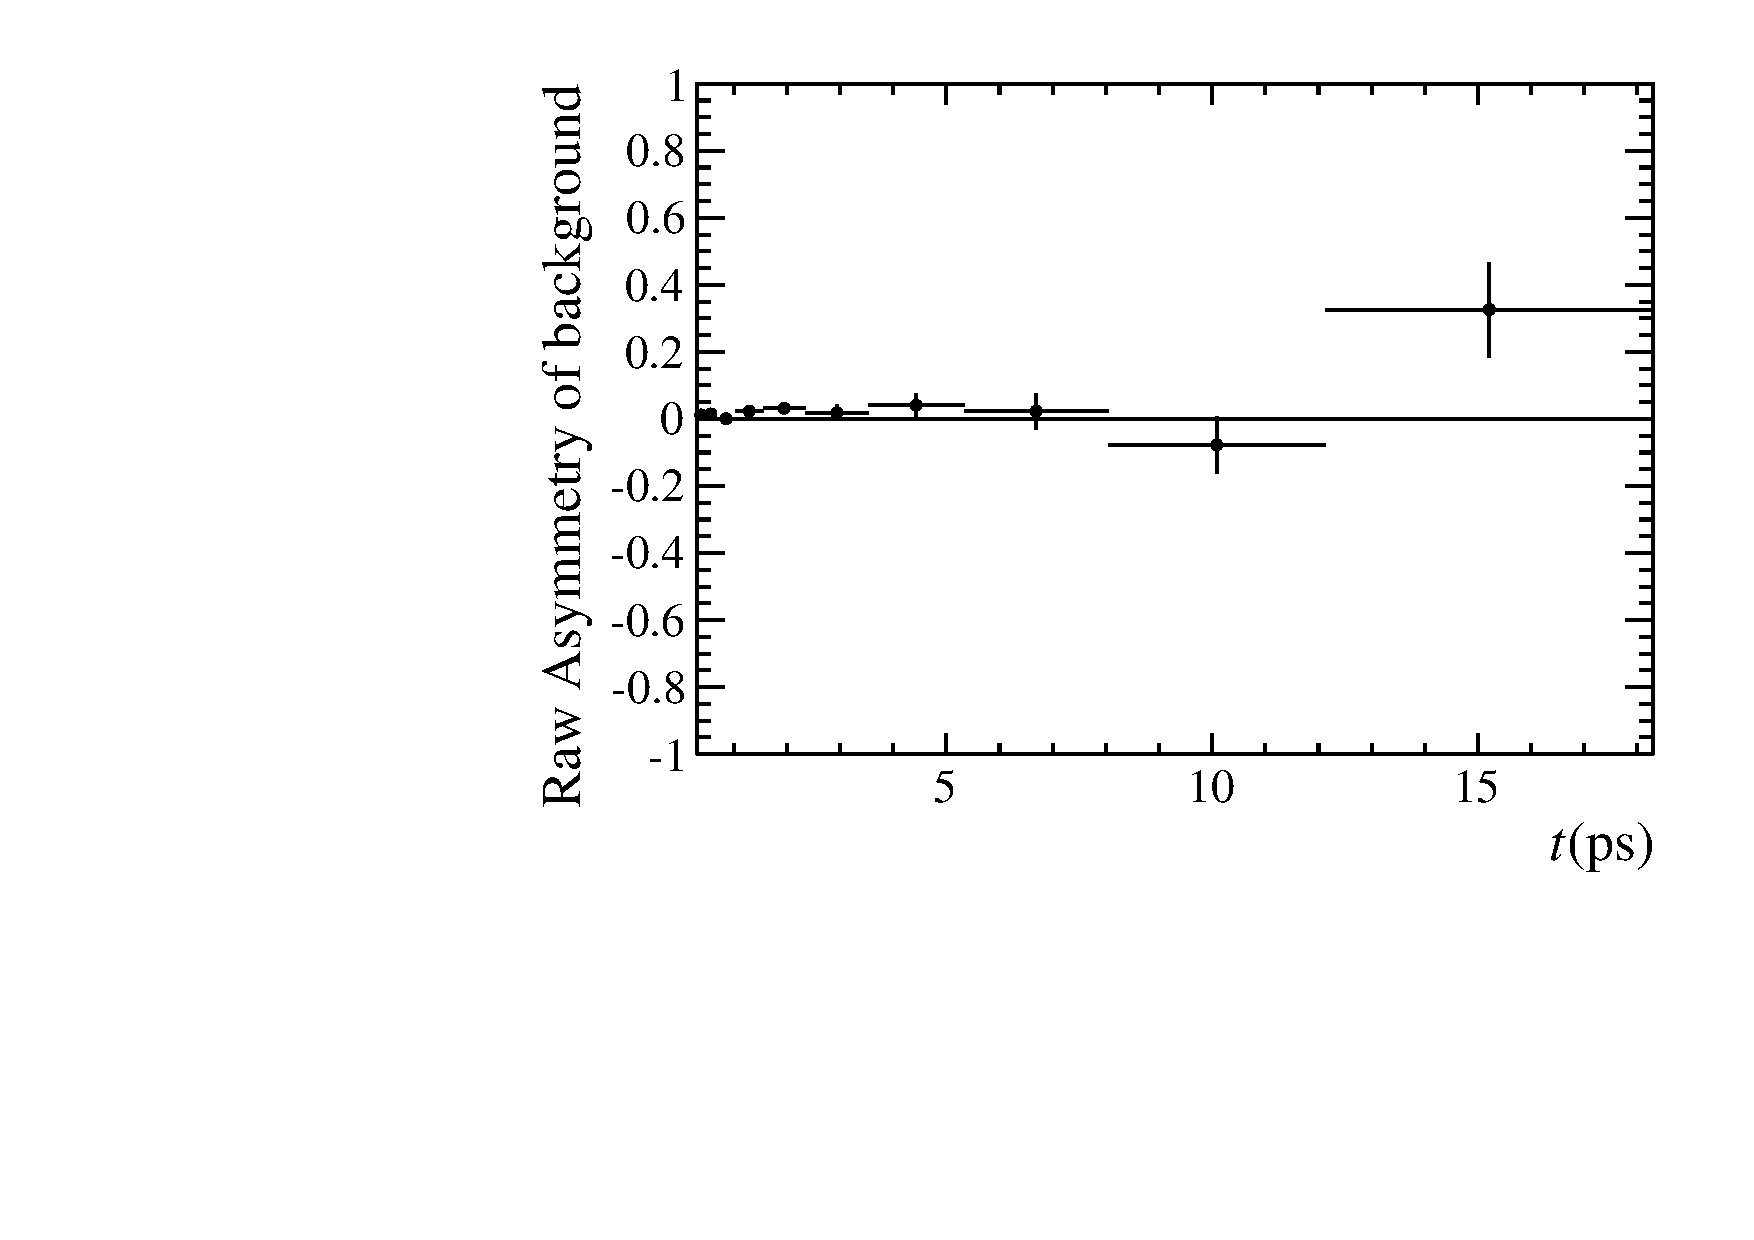
\includegraphics[width=0.49\textwidth]{private/content/measurement-of-sin2beta/figs/tagged_bkg_data_dd_os.pdf}
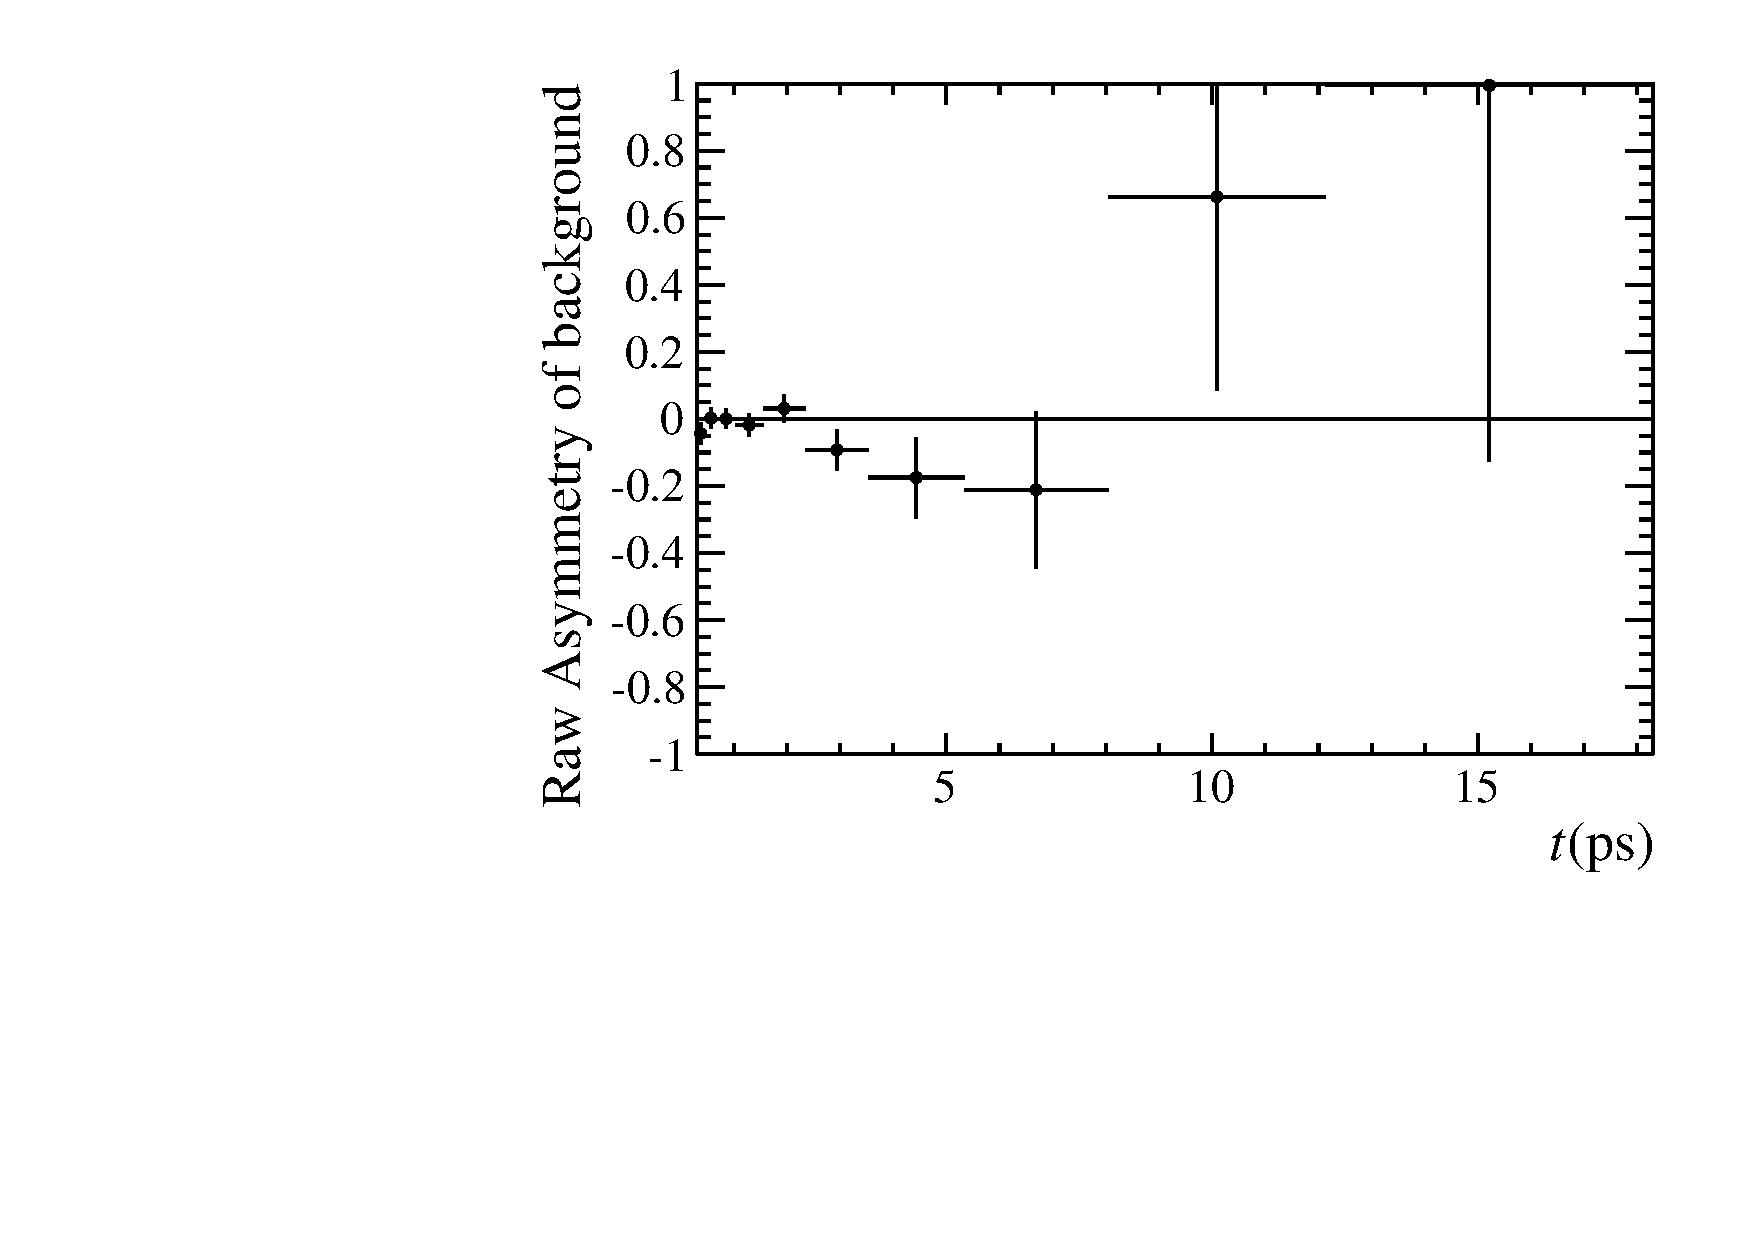
\includegraphics[width=0.49\textwidth]{private/content/measurement-of-sin2beta/figs/tagged_bkg_data_dd_ss.pdf}
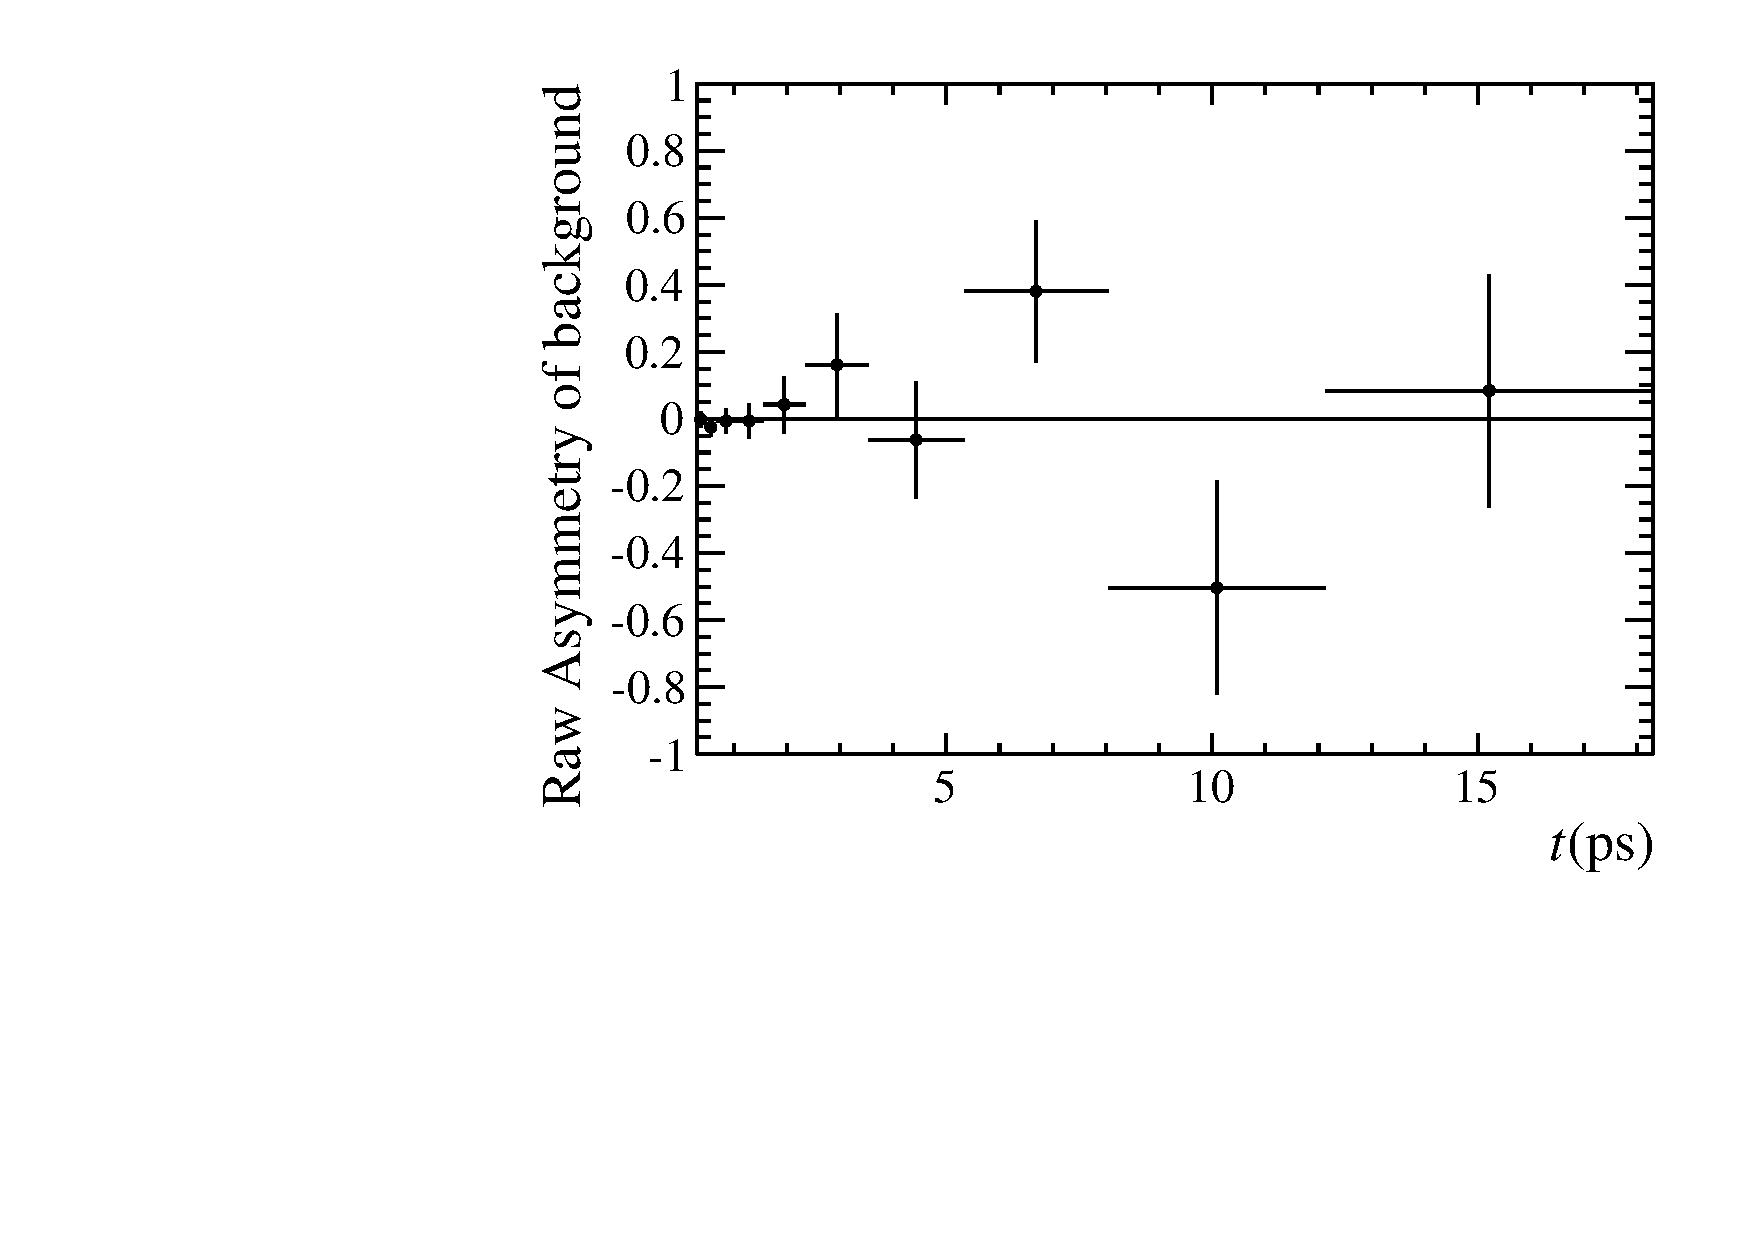
\includegraphics[width=0.49\textwidth]{private/content/measurement-of-sin2beta/figs/tagged_bkg_data_ll_os.pdf}
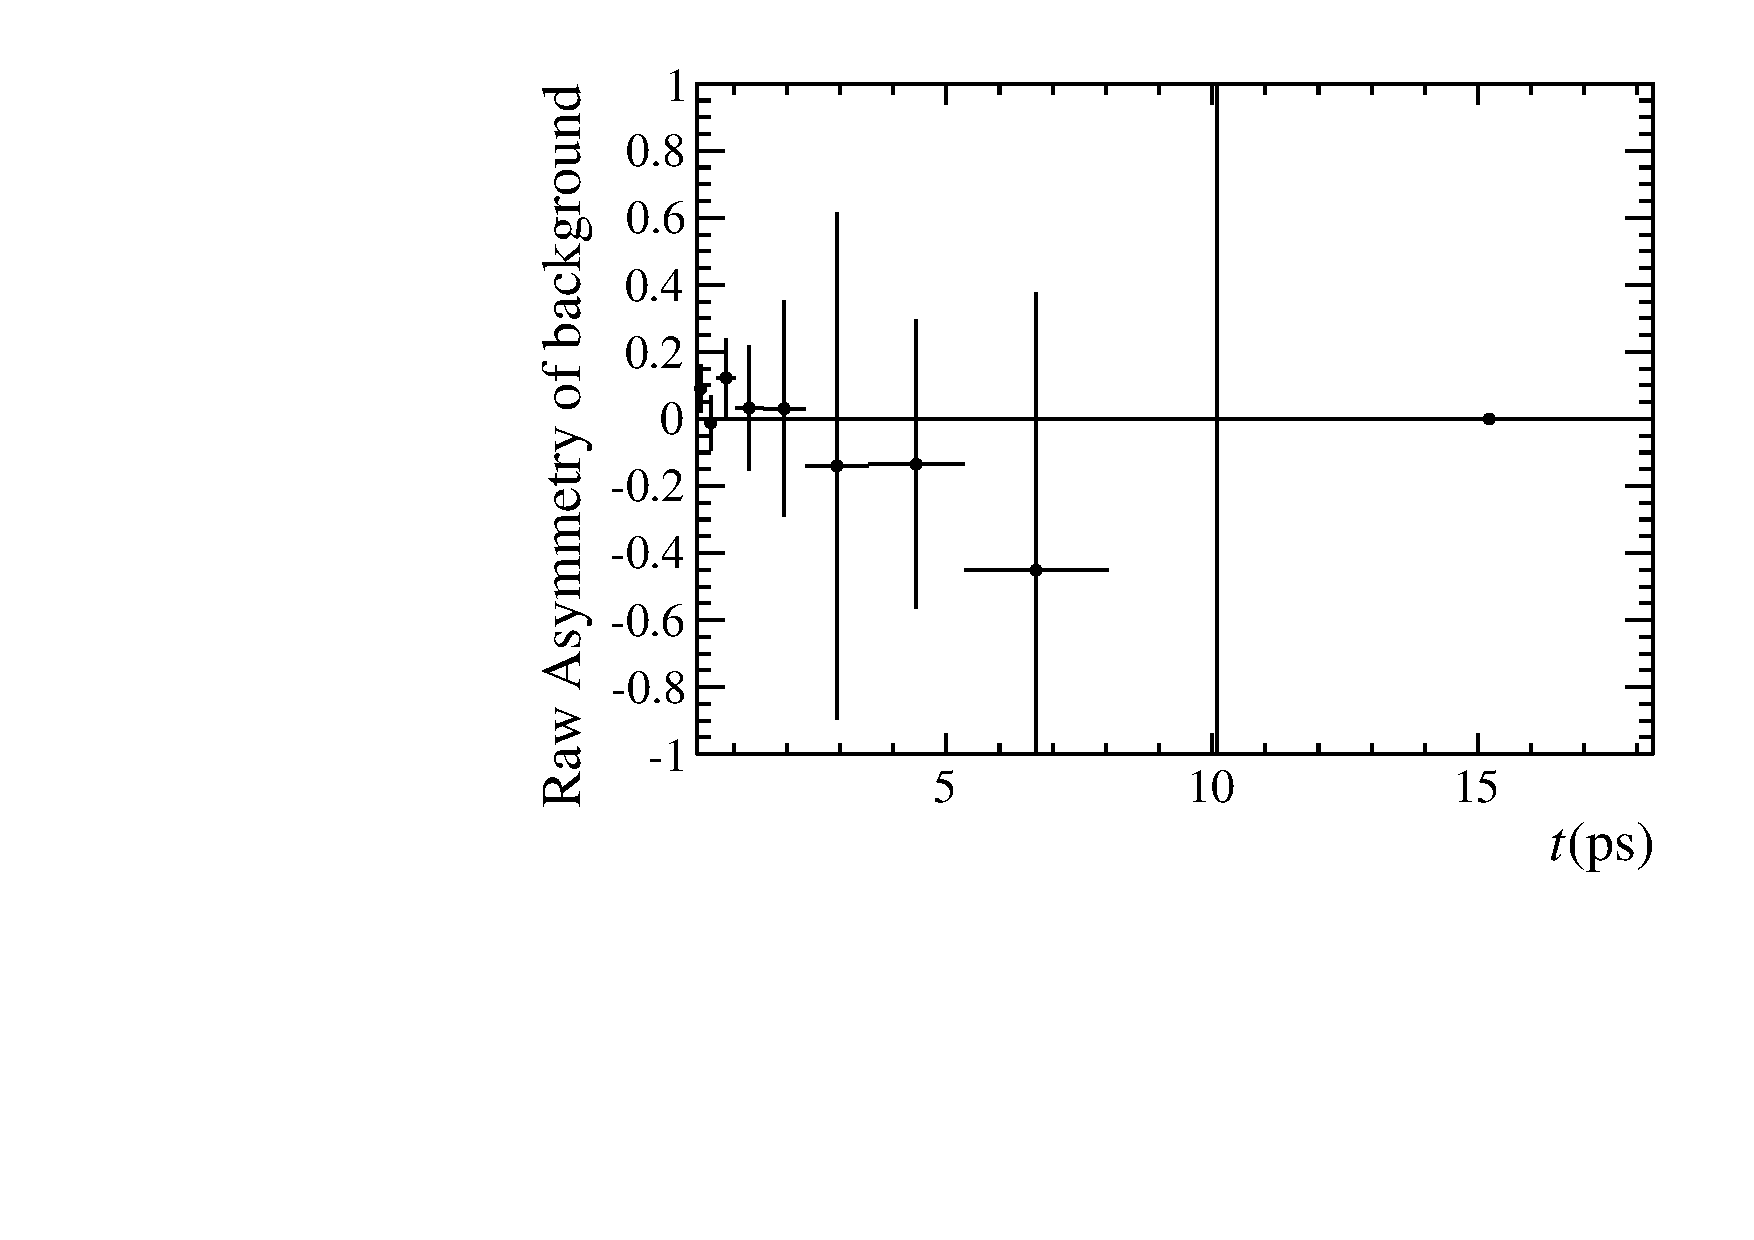
\includegraphics[width=0.49\textwidth]{private/content/measurement-of-sin2beta/figs/tagged_bkg_data_ll_ss.pdf}
\caption{Tagging asymmetry $\Asym{}{}(\obsTime)$ in background \sweighted data.
The binning of the $x$-axis is chosen logarithmic. The top (bottom) plots show
\catDD (\catLL) candidates, while \OS (\SSpi) tagged candidates are depicted in
the left (right) side.}
\label{fig:measurement_of_sin2beta:physic_backgrounds:tagging_asymmetries:data}
\end{figure}
%
\begin{figure}[h]
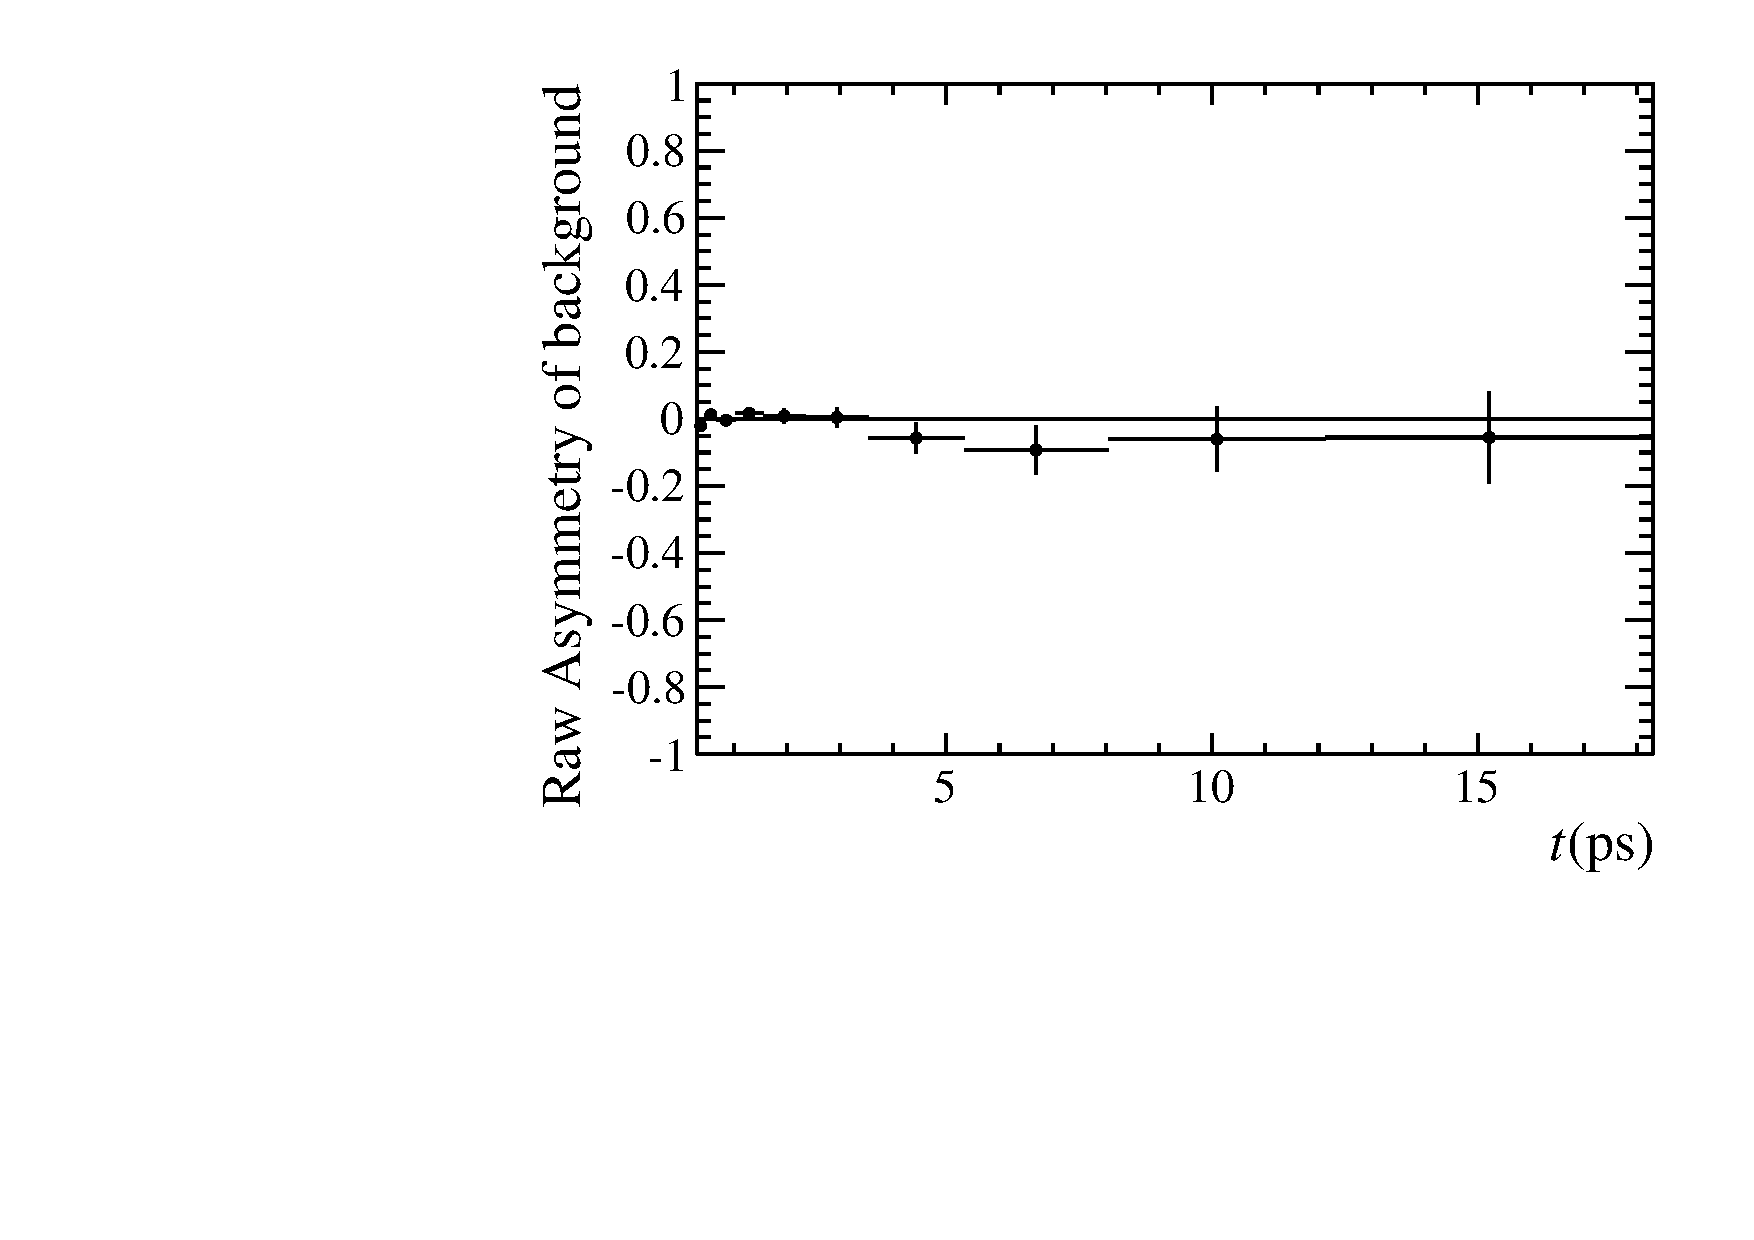
\includegraphics[width=0.49\textwidth]{private/content/measurement-of-sin2beta/figs/tagged_bkg_toymc_dd_os.pdf}
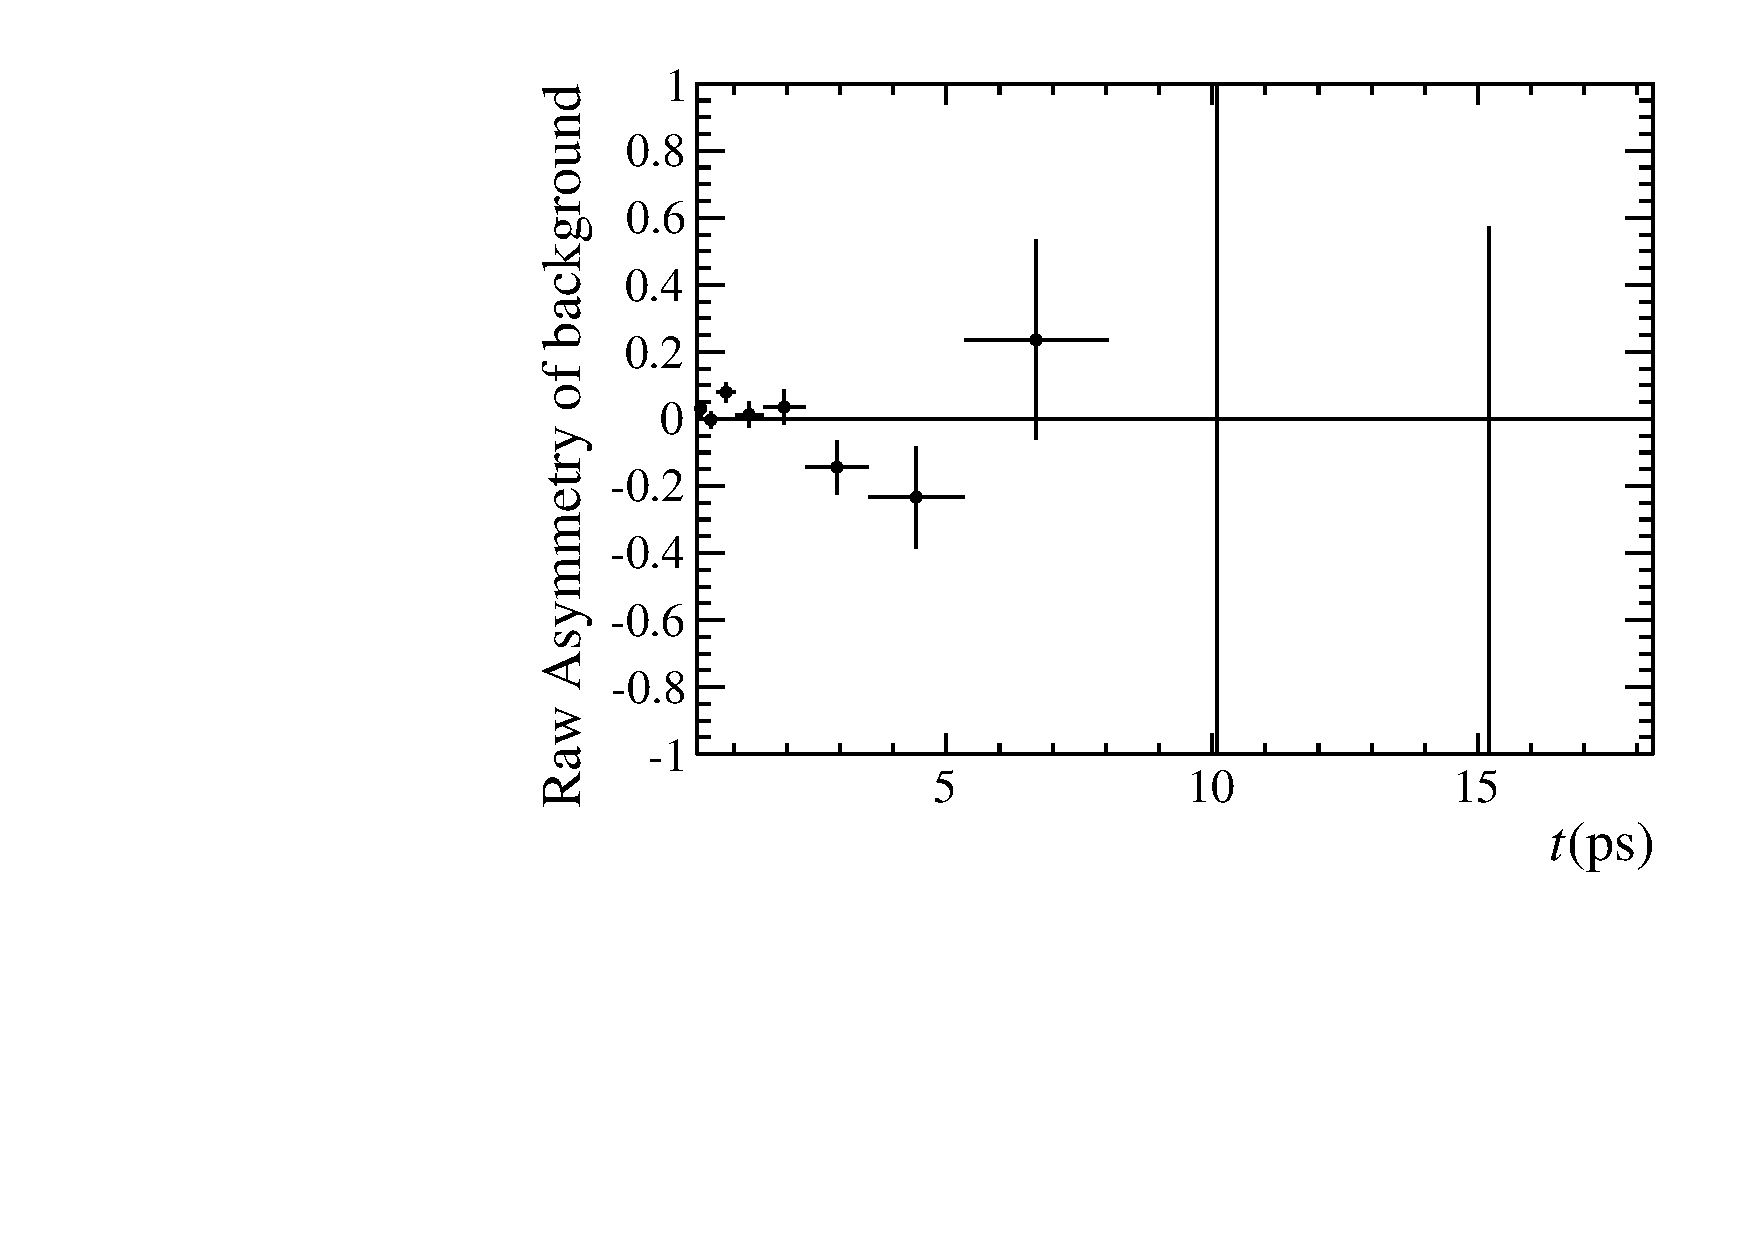
\includegraphics[width=0.49\textwidth]{private/content/measurement-of-sin2beta/figs/tagged_bkg_toymc_dd_ss.pdf}
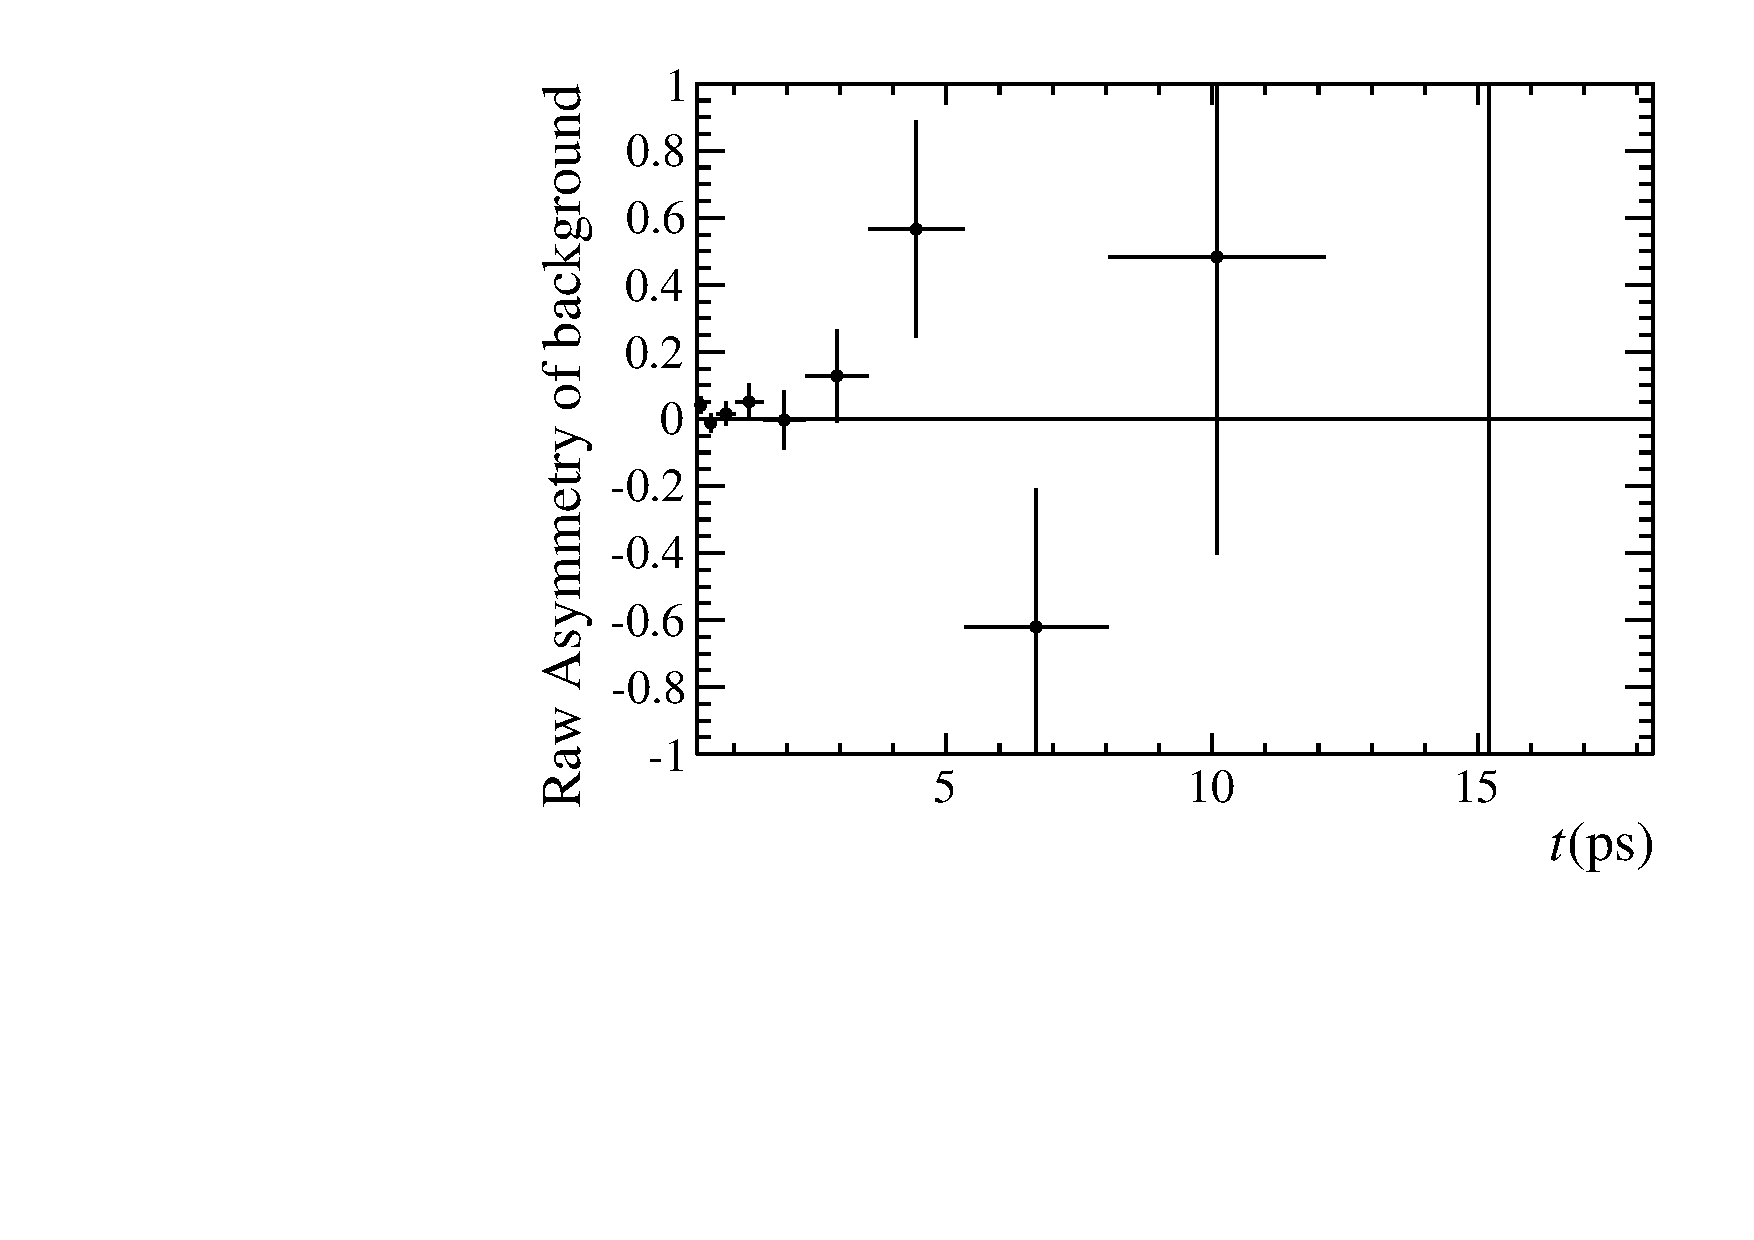
\includegraphics[width=0.49\textwidth]{private/content/measurement-of-sin2beta/figs/tagged_bkg_toymc_ll_os.pdf}
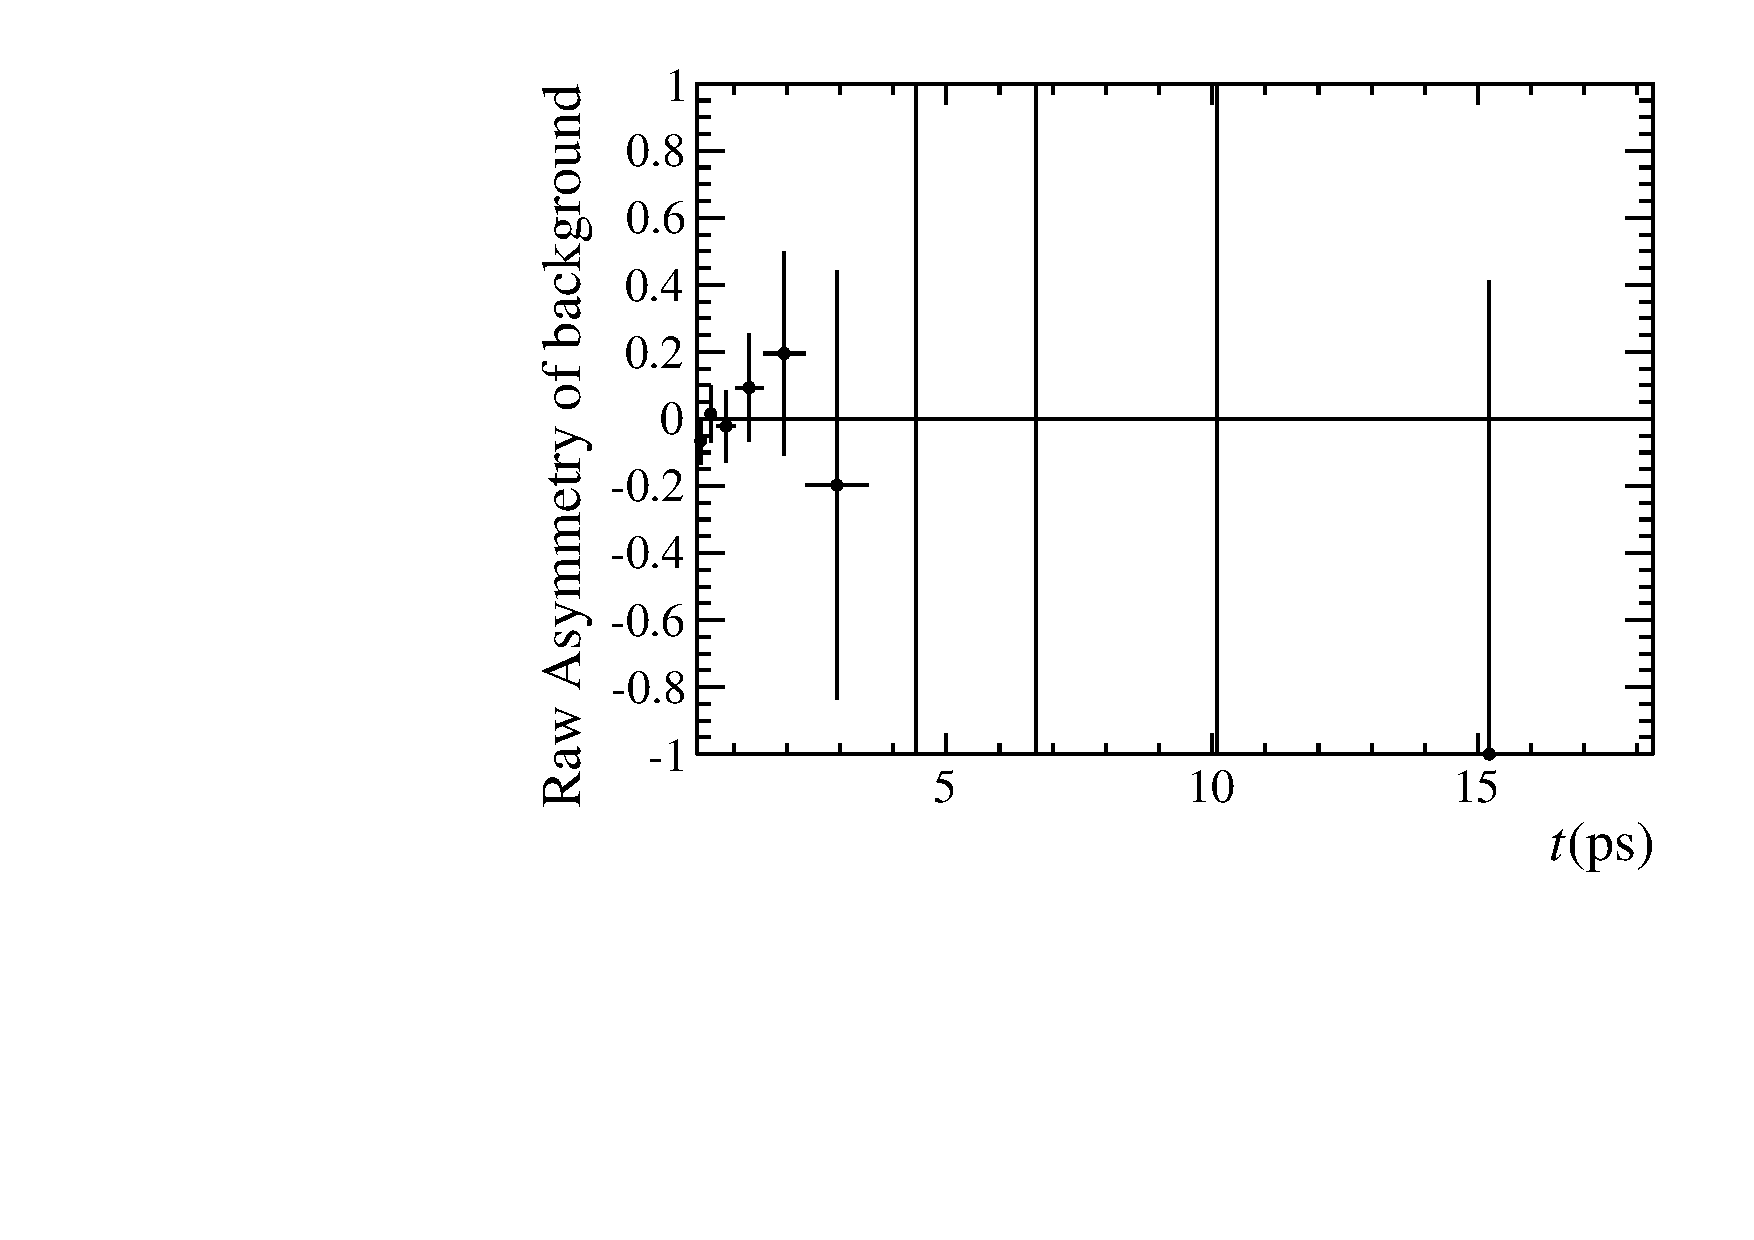
\includegraphics[width=0.49\textwidth]{private/content/measurement-of-sin2beta/figs/tagged_bkg_toymc_ll_ss.pdf}
\caption{Tagging asymmetry $\Asym{}{}(\obsTime)$ in cocktail \MC with signal
candidates taken from \BdToJpsiKS signal \MC and background candidates from a
\ToyMC sample. The binning of the $x$-axis is chosen logarithmic. The top
(bottom) plots show \catDD (\catLL) candidates, while \OS (\SSpi) tagged
candidates are depicted in the left (right) side.}
\label{fig:measurement_of_sin2beta:physic_backgrounds:tagging_asymmetries:toymc}
\end{figure}

\paragraph{A likelihood fit} to the \sweighted background candidates is
conducted in order to exploit the per-event tag information. To do so the
distributions are fitted using a \ac{PDF} as presented in
\cref{eq:measurement_of_sin2beta:physic_backgrounds:tagging_asymmetries:time_dependent:pdf} 
where a potential asymmetry has been modelled. The parametrisation uses
the sum of three (two in case of the \catDD \SSpi subsample) exponential
\acp{PDF} with independent pseudo-lifetimes $\tau_i$ and individual asymmetry
parameters $\Asym{i}{}$.
%
\begin{table}[h]
\centering
\caption{Fit results of the asymmetries $\Asym{i}{}$ of a fit to the \sweighted
background distributions of \catDD and \catLL \OS and \SSpi tagged events.}
\label{sec:measurement_of_sin2beta:physic_backgrounds:tagging_asymmetries:time_dependent:likelihood:results}
\sisetup{
  table-number-alignment    = center,
  table-figures-integer     = 1,
  table-figures-decimal     = 3,
  table-figures-uncertainty = 3,
  table-sign-mantissa,
}
\begin{tabular}{
  llSS
  S[
    table-figures-decimal     = 2,
    table-figures-uncertainty = 2,
  ]}
\toprule
\multicolumn{2}{c}{category}  &   {$\Asym{1}{}$}  & {$\Asym{2}{}$}  & {$\Asym{3}{}$} \\
\midrule
\catDD & \acs*{OS}            &    0.001 +- 0.028 & -0.039 +- 0.030 & -0.01 +- 0.07 \\
\catDD & \acs*{SSpi}          &   -0.01  +- 0.04  &  0.14  +- 0.14  & {---}         \\
\catLL & \acs*{OS}            &    0.05  +- 0.05  & -0.03  +- 0.13  & -0.11 +- 0.12 \\
\catLL & \acs*{SSpi}          &   -0.01  +- 0.20  & -0.18  +- 0.18  &  0.4  +- 0.4  \\
\bottomrule
\end{tabular}
\end{table}

\paragraph{A final conclusion} on how to proceed is difficult as the results are
inconclusive due to a lack of statistical power. Although all results are
compatible with the hypothesis of a vanishing background tagging asymmetry,
there is evidence of non-vanishing asymmetries supported by fluctuations found
in the results.

Thus, the nominal fit model does not incorporates a description of a potential
tagging asymmetry in the background component. The impact of this decision is
further investigated in a \ToyMC study presented in
\cref{sec:measurement_of_sin2beta:systematics:systematics:fit_model}
